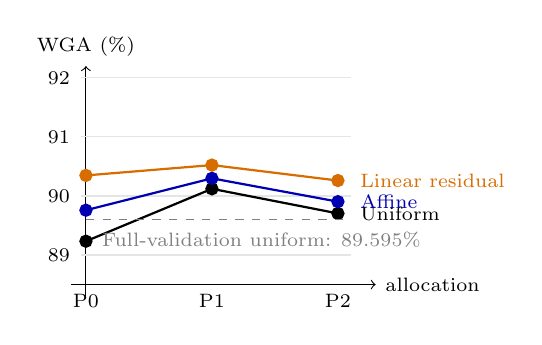
\begin{tikzpicture}[x=1.6cm,y=0.75cm,font=\scriptsize]
\draw[->] (-0.12,0) -- (2.3,0) node[right]{allocation};
\draw[->] (0,-0.2) -- (0,3.7) node[above]{WGA (\%)};
\draw[gray!20] (-0.04,0.5) -- (2.1,0.5);
\node[left] at (-0.05,0.5) {89};
\draw[gray!20] (-0.04,1.5) -- (2.1,1.5);
\node[left] at (-0.05,1.5) {90};
\draw[gray!20] (-0.04,2.5) -- (2.1,2.5);
\node[left] at (-0.05,2.5) {91};
\draw[gray!20] (-0.04,3.5) -- (2.1,3.5);
\node[left] at (-0.05,3.5) {92};
\node[below] at (0,0) {P0};
\node[below] at (1,0) {P1};
\node[below] at (2,0) {P2};
\draw[thick,black] plot[mark=*] coordinates {(0,0.73373) (1,1.62131) (2,1.20439)};
\node[right,black] at (2.1,1.20439) {Uniform};
\draw[thick,blue!70!black] plot[mark=*] coordinates {(0,1.25881) (1,1.79862) (2,1.40383)};
\node[right,blue!70!black] at (2.1,1.40383) {Affine};
\draw[thick,orange!85!black] plot[mark=*] coordinates {(0,1.84780) (1,2.02310) (2,1.76106)};
\node[right,orange!85!black] at (2.1,1.76106) {Linear residual};
\draw[dashed,gray] (0,1.095) -- (2.05,1.095);
\node[gray,anchor=west] at (0.05,0.75) {Full-validation uniform: 89.595\%};
\end{tikzpicture}